\section{Используемые технологии и приёмы программирования}

В данном разделе будет приведено описание языков программирования, фреймворков,
используемых при разработке, и базы данных, применяемой в программе, а также
изложен подход, применяемый к проектированию архитектуры приложения.

\subsection{Язык программирования \kt{}}
\label{sec:kt}

\kt{} (Котлин) --- статически типизированный язык программирования, работающий поверх 
JVM и разрабатываемый компанией JetBrains.

Основные приемущества языка \kt{}:
\begin{itemize}
  \item краткость --- кострукции и возможности языка разрабатывались с целью уменьшить 
  количество кода, но при этом не уменьшая читаемости этого кода;
  \item поддержка защиты от NullPointerException на уровне языка;
  \item полная совместимость с языком программирования Java, что позволяет использовать
  весь набор библиотек и технологий, накопленных за долгое время существования Java;
  \item возможность расширять библиотеки, не изменяя их код, что позволяет дописывать необходимую 
  функциональность без нарушений каких-либо лицензий либо поиска исходников уже 
  скомпилированных библиотек (листинг \ref{lst:kt_ext});
  \item мультипарадигмость --- \kt{} можно писать код как в процедурном стиле, так и в 
  объектно-ориентированном, а также благодаря поддержке функций высшего порядка можно 
  писать код и в функциональном стиле. Сочетание лучших качеств у каждого из этих стилей 
  позволяет разрабатывать приложения быстро и эффективно (листинг \ref{lst:kt_map});
\end{itemize} 

\begin{lstlisting}[style = ktstyle, 
           caption = {Пример Extension-функции на языке \kt{}},
           label = {lst:kt_ext}]
public fun CharSequence.padEnd(length: Int, padChar: Char = ' '): CharSequence {
    if (length < 0)
        throw IllegalArgumentException("Desired length $length is less than zero.")
    if (length <= this.length)
        return this.subSequence(0, this.length)

    val sb = StringBuilder(length)
    sb.append(this)
    for (i in 1..(length - this.length))
        sb.append(padChar)
    return sb
}
\end{lstlisting}

\begin{lstlisting}[style = ktstyle, 
           caption = {Реализация популярной функции высшего порядка <<map>> на языке \kt{}},
           label = {lst:kt_map}]
fun <T, R> List<T>.map(transform: (T) -> R): List<R> {
    val result = arrayListOf<R>()
    for (item in this)
        result.add(transform(item))
    return result
}
\end{lstlisting}



\subsection{Шаблон проектирования \mvc{}}

Достаточно часто в процессе разработки требуется вносить изменения в логику
работы программы. Любые видоизменения в логике влекут за собой изменения в
исходном коде. Как известно, при модификации исходного кода есть риск допустить
ошибку. Очевидно, что программирование без изменения исходного кода невозможно,
однако при проектировании архитектуры программы следует делать это так, чтобы
переписывать как можно меньше кода при внесении изменений в логику работы. Иными
словами, архитектура должна быть гибкой и расширяемой.

Паттерн проектирования --- это идея решения проблемы проектирования в
определенном, характерном контексте. Таким образом, само решение проблемы, то
есть реализация какого-либо паттерна на языке программирования, все еще является
задачей для разработчика, однако шаблон определяет некоторые аспекты отношения и
взаимодействия между классами и объектами, снижая сложность разработки.

Шаблон проектирования \mvc{} --- это популярный подход к построению архитектуры
приложения, когда модель приложения, интерфейс и взаимодействие с пользователем
разделены на три отдельных компонента таким образом, чтобы модификация одного из
компонентов оказывала минимальное воздействие на остальные (рисунок
\ref{fig:mvc}).

Основная цель применения этой концепции состоит в отделении модели от её
представления. За счет такого разделения повышается возможность повторного
использования кода. Наиболее полезно применение данной концепции в тех случаях,
когда пользователь должен видеть те же самые данные одновременно в различных
контекстах. Например, некоторые данные могут быть одновременно представлены в
виде электронной таблицы, гистограммы и круговой диаграммы.
Данный подход также упрощает совместную разработку, так как позволяет каждой
команде разработчиков концентрироваться только на своей задаче.
Поэтому возможно добиться того, что программисты, занимающиеся разработкой
бизнес-логики (<<модели>> в терминах MVC), вообще не будут осведомлены о том,
какое представление будет использоваться.

\begin{figure}[h!]
\centering
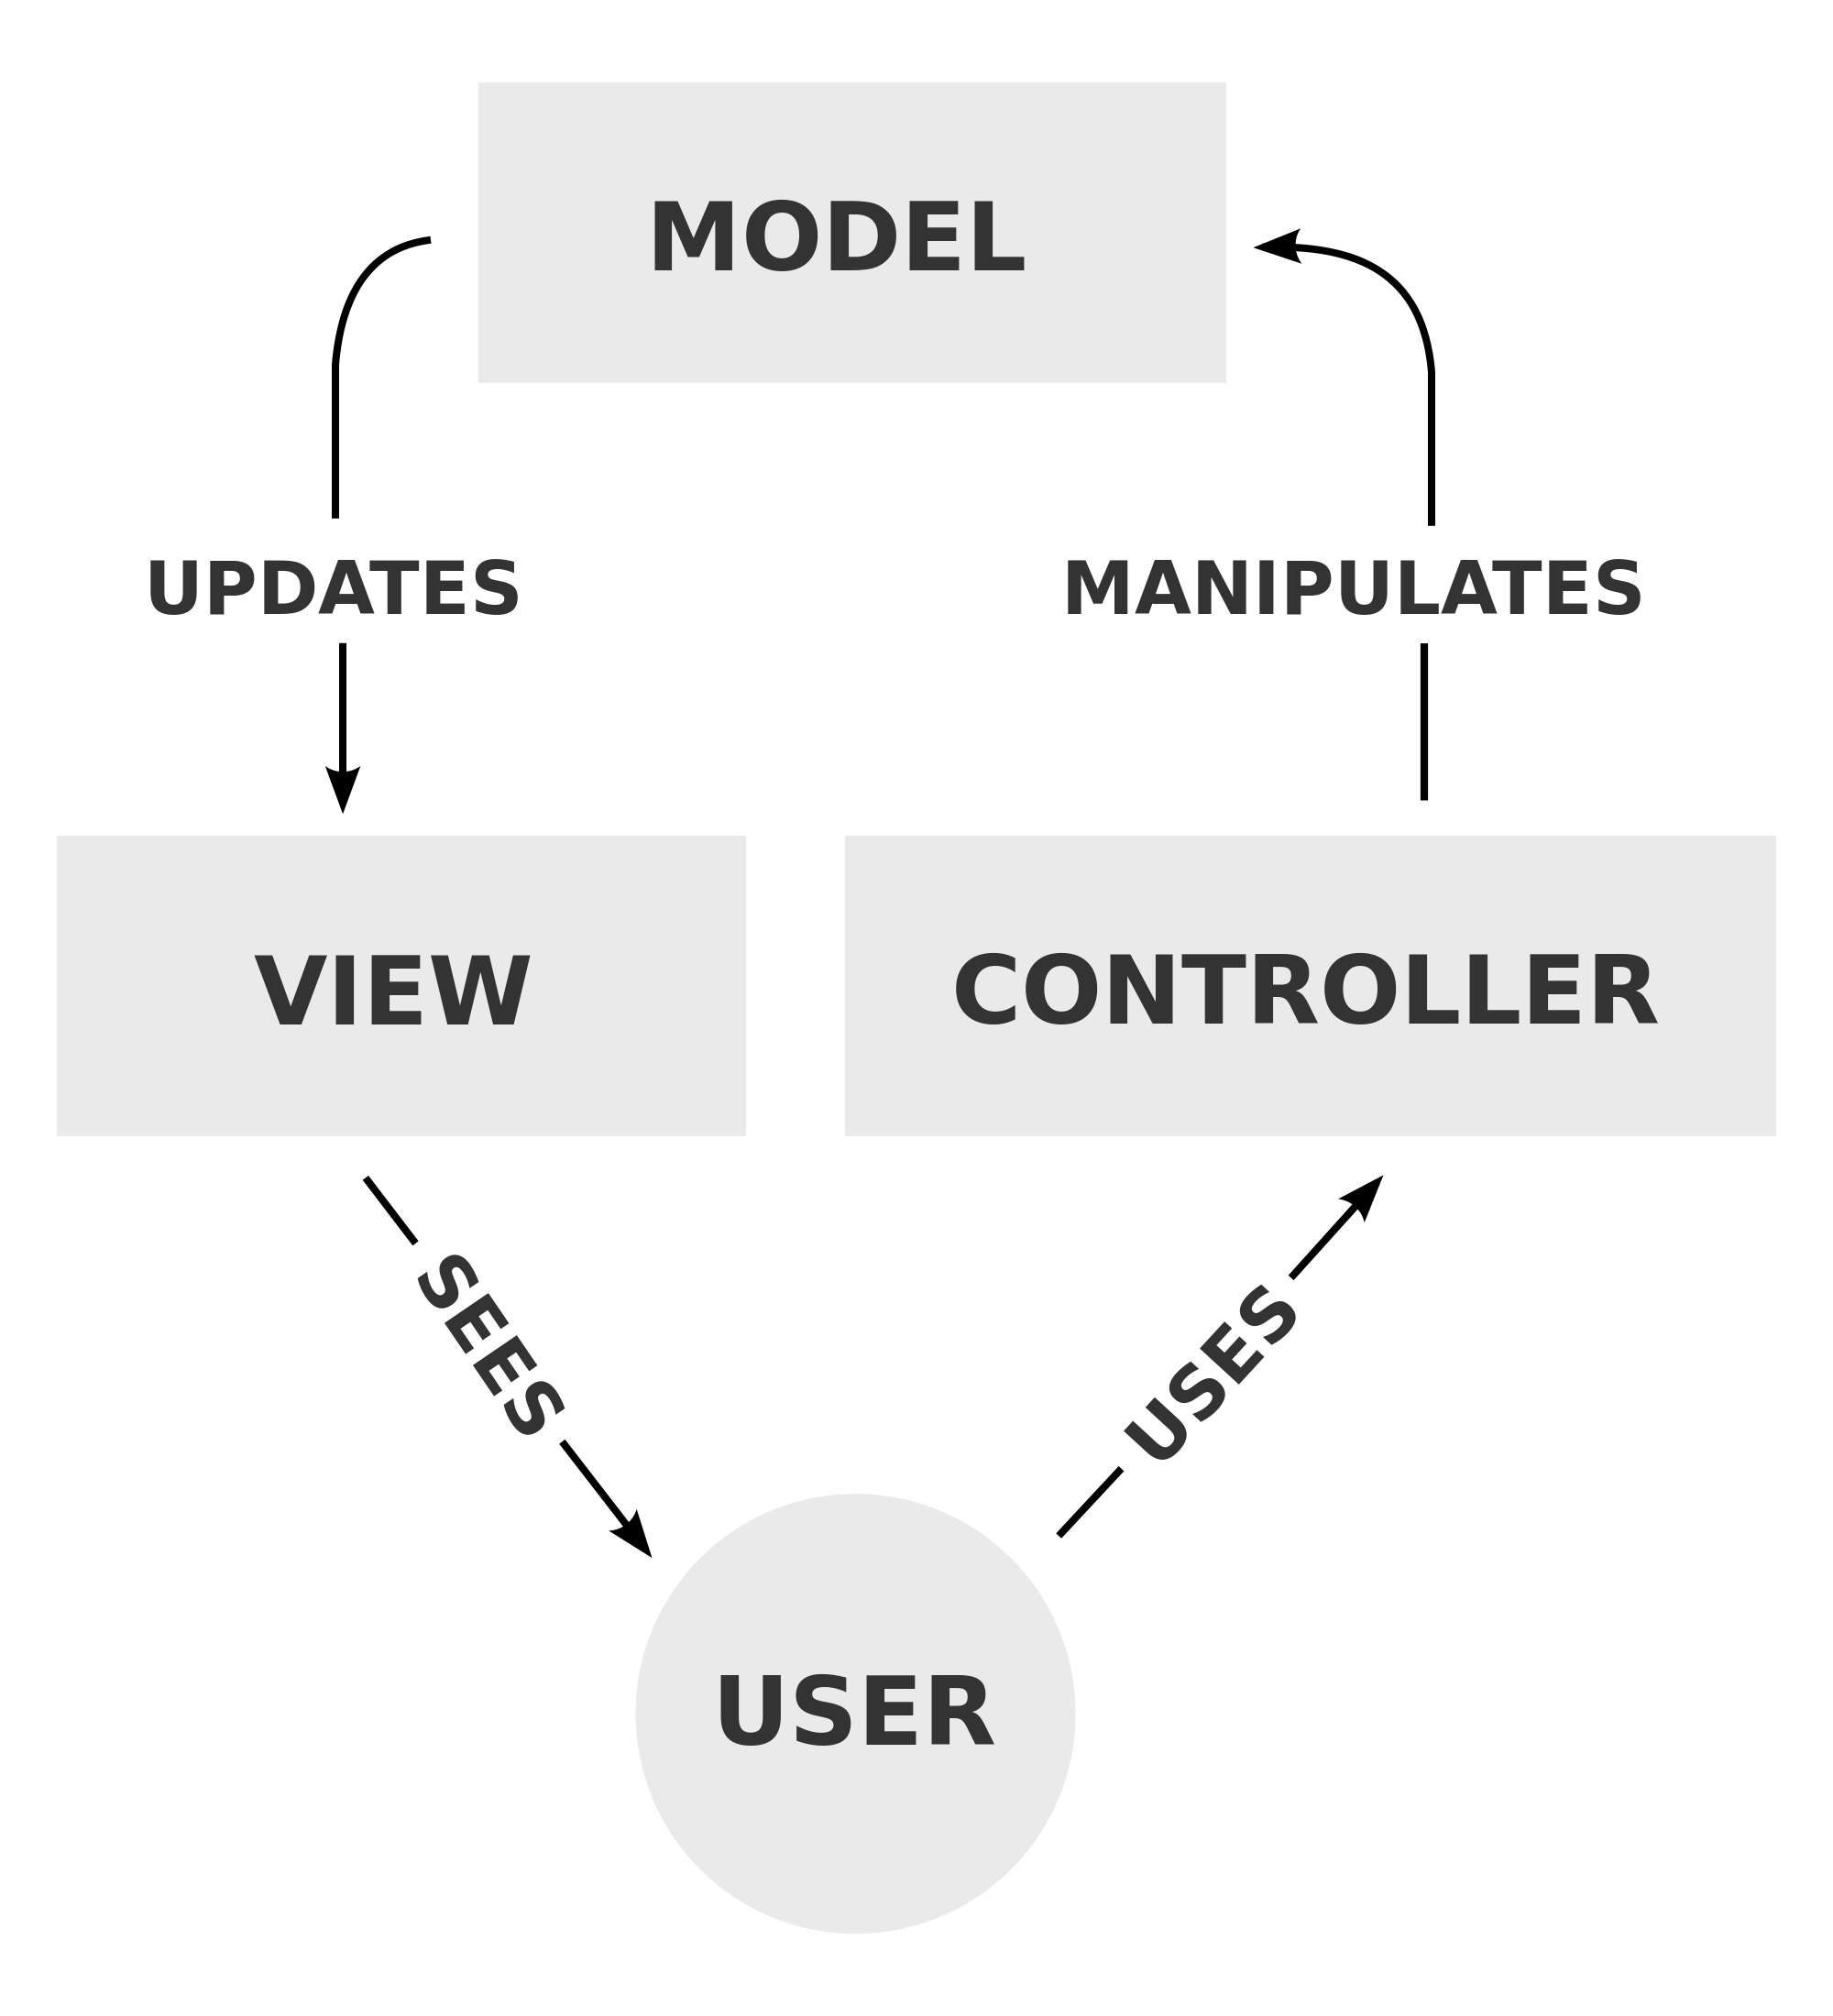
\includegraphics[scale = 0.15]{mvc.png}
\caption{Схема взаимодействия компонентов MVC}
\label{fig:mvc}
\end{figure}

При правильном применении \mvc{} существенно облегчает поддержку программы и
снижает затраты на изменение или добавление функциональности.

\subsection{База данных SQLite}
\label{sec:sqlite}
Процесс загрузки большого количества данных через запросы с API может занять
достаточно продолжительное время. Даже несмотря на возможность одновременной
загрузки данных и вывода уже загруженных, необходимо минимизировать расход
трафика и нагрузку на сеть в процессе работы с приложением путем кэширования
уже загруженных данных и периодического обновления кэша по мере появления новой
информации на сервере.

Для этих целей отлично подойдет встраиваемая реляционная база данных SQLite.
Данная база данных не использует клиент-серверную архитектуру, то есть не имеет
отдельно работающего процесса, взаимодействующего с клиентской программой и
базой данных, а предоставляет библиотеку, с которой программа компонуется. Таким
образом движок становится составной частью программы. SQLite хранит всю базу
данных в единственном файле, что уменьшает накладные расходы, время отклика и упрощает
программу.

Несколько процессов или потоков могут одновременно без каких-либо проблем читать
данные из одной базы. Запись в базу можно осуществить только в том случае, если
никаких других запросов в данный момент не обслуживается; в противном случае
попытка записи оканчивается неудачей, и в программу возвращается код ошибки.

SQLite отличается простотой использования и встраивания, в связи с чем активно
используется во многих популярных приложениях.




